\chapter{Tekniska specifikationer}
\label{chap:tech}
SALSA Onsala är en modifierat TV-antenn med diameter 2.3~m som är utvecklad
för mätningar vid frekvensen 1420\,MHz.

\section{Vinkelupplösning och precision}
\label{sect:ares}
SALSA har en vinkelupplösning på ca 6$^\circ$ (\emph{full width half
maximum}) vid 1420\,MHz. Detta värde har uppmätts genom observationer av solen,
se Fig. \ref{fig:beam}. För att jämföra, kom ihåg att fullmånen har en
vinkelutsträckning på ca en halv grad, eller 30 bågminuter. Motorerna trackar
i steg om 0.125$^\circ$, och detta är alltså teleskopets precision vid ideala
förhållanden. Men, om det är blåsigt\footnote{Du kan kolla hur mycket det blåser
vid SALSA just nu på http://wx.oso.chalmers.se/weather/} så kan teleskopet
röra sig lite i vinden (kring den önskade positionen) och då störa riktningen på
teleskopet under små tidsintervall med ca 1-2 $^\circ$. Detta bör dock inte vara
något problem för användare då rörelserna från vinden är mindre än teleskopets
vinkelupplösning.
\begin{figure}[ht]
\begin{center}
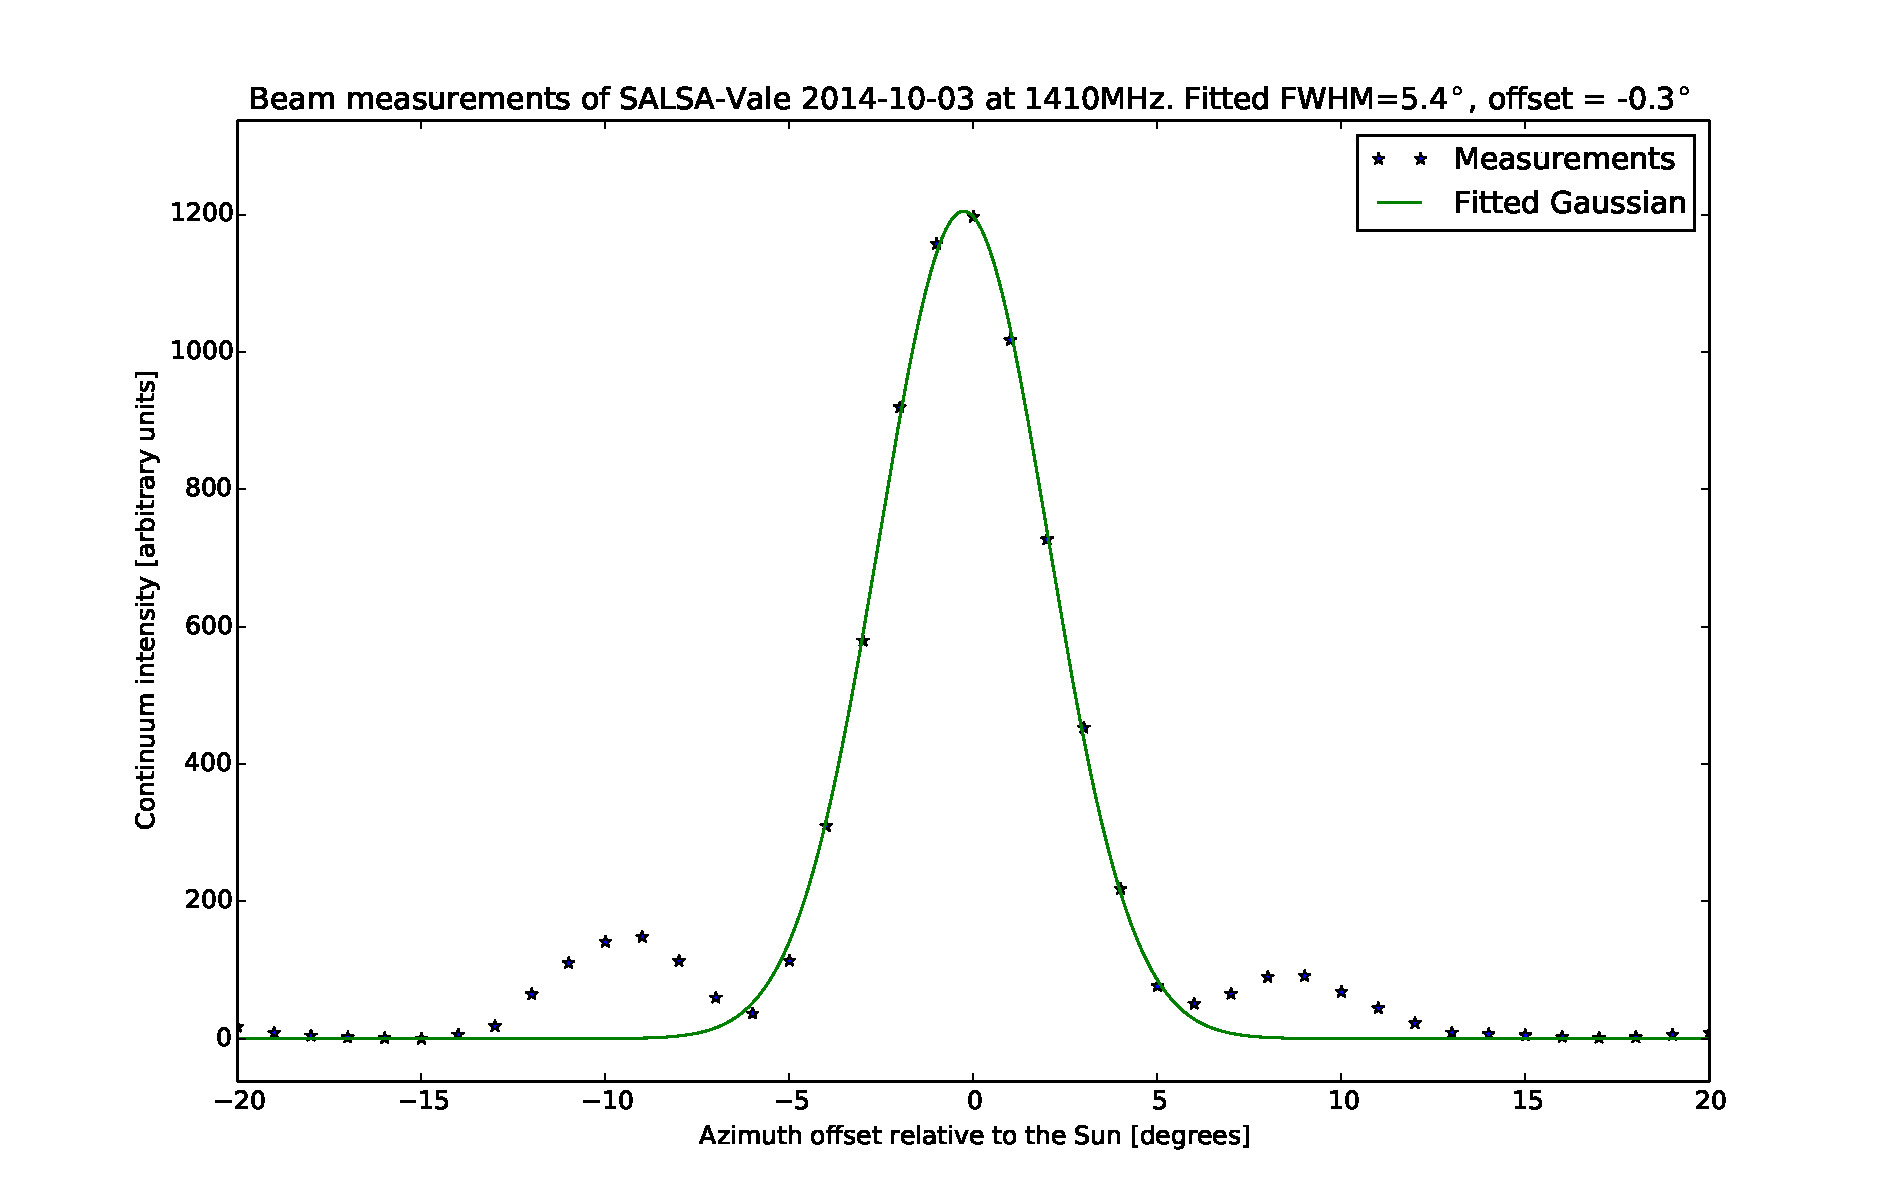
\includegraphics[width=\textwidth]{../figures/Beam_vale_2014-10-03.pdf}
\end{center}
\caption{Antennresponsen för telskopet Vale uppmätt med Solen vid 1410\,MHz. 
	En gaussisk anpassning ger FWHM=5.4$^\circ$. Sidloberna av Sinc-function 
	kan ses tydligt, precis som väntat för en cirkulär apertur. }
\label{fig:beam}
\end{figure}

\section{Frekvensupplösning och precision}
SALSA använder enheten \emph{Universal Software Radio Peripheral} (USRP) för
att göra mätningar. Denna USRP fungerar som en sampler som spelar in en
tidsserie till hårddisken på kontrolldatorn. Kanaliserandet, alltså bildandet
av ett spektrum, görs genom mjukvara (FFT). Detta innebär att antalet kanaler
inte är fixerat, och inte heller bandbrädden. Frekvensupplösningen är begränsad
av ledigt hårddiskutrymme och beräkningskapaciteten hos kontrolldatorn. Upp
till 10\,MHz bandbredd med 8192 kanaler har testats, men för de flesta
observationer så räcker det utmärkt med standardinställningarna på 2\,MHz
bandbredd och 256 kanaler, d.v.s. en frekvensupplösning på 7.8\,kHz per kanal.
Om en högre upplösning krävs så kan det väljas under fliken \emph{Advanced} i
rutan \emph{Receiver control} i kontrollprogrammet, men vi erbjuder i skrivande
stund ingen support för dessa avancerade inställningar. 

\section{Fluxkalibrering och osäkerhet}
SALSA är för närvarande INTE NOGGRANNT FLUXKALIBRERAT. Detta innebär att SALSA endast ska användas till att mäta HI-hastigheter, inte HI-antenna temperaturer. Vi planerar att kalibrera SALSA i framtiden, men teleskopet genomgår fortfarande förändringar vilket gör det opraktiskt att kalibrera det nu. När det är kalibrerat så kommer denna manual att uppdateras med relevant informarion. 
